\chapter{BIBO Stability of systems}\label{chap:stability}

A system is said to be bounded-input, bounded output stable (BIBO stable) if,
given a bounded input, it produces a bounded output. In this lab you will be
using \textsf{Matlab} and \textsf{Simulink} to examine the BIBO stability of
several systems.

\section{Prelab}

Before you go into the lab, you should read the following:
\begin{itemize}
\item Sections 5.1 and 5.2 of the course notes on
system stability.
\end{itemize}

\section{Procedure}

In this part of the lab, you are given three different control systems.  For
each system you will prepare a \textsf{Simulink} model to analyze the outputs
of the system to various bounded inputs, and examine their ``impulse
response'' (even keeping in mind that the true impulse response is a physical
impossibility).
\begin{enumerate}
\item Consider the linear system:
\begin{eqnarray*}
\dot{\vect{x}}&=&\begin{bmatrix}0&1\\-1&0\\\end{bmatrix}\vect{x}
\begin{bmatrix}0\\1\end{bmatrix}u\\
y&=&\begin{bmatrix}1&0\end{bmatrix}\vect{x}
\end{eqnarray*}
and determine $(\mat{A},\vect{b},\vect{c}^{t},\mat{D})$\@.

\item Use the \verb|impulse| command in \textsf{Matlab} to produce the
impulse response of the system (recall that
$h_{\Sigma}(t)=\vect{c}^{t}\eul^{\mat{A}t}\vect{b}$). Comment on the feature
of the impulse response that determines BIBO stability. Do you expect the
system to be BIBO stable?

\item You can calculate the transfer function in several ways: take the
Laplace transform of the impulse response, noting that the systems you are
given are all in controller canonical form; using the \verb|tf| command in
\textsf{Matlab}\@.  Choosing whichever method you like, calculate the
transfer function, and comment on its poles. Is this consistent with your
prediction of BIBO stability?

\item Prepare the \textsf{Simulink} model shown in Figure~\ref{fig:model5}\@.
\begin{figure}[htbp]
\centering
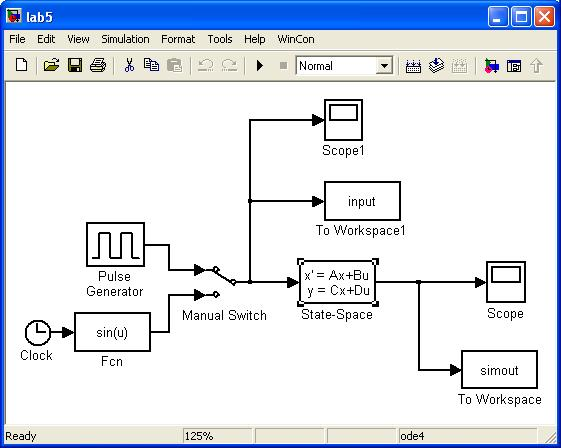
\includegraphics[width=0.6\hsize]{pix/model5.jpg}
\caption{\textsf{Simulink} model for Lab~\ref{chap:stability}}        \label{fig:model5}
\end{figure}%
You could use the model in Lab~\ref{chap:impulseresponse} if you saved it.
They are the same.

\item If you determined that the system is not BIBO stable, modify your
\textsf{Simulink} model by replacing the \verb|Pulse Generator| with the
\verb|Fcn| block and specifying a bounded input that will produce an
unbounded output.  If the system was determined to be BIBO stable, give the
system any bounded input you desire.  In either case, print a plot of the
output variable $y$ and the input variable $u$\@.

\item We will now examine the impulse response of the system.  You can use
the same \textsf{Simulink} model generated above and proceed as in
Lab~\ref{chap:impulseresponse}\@.  Recall that the \verb|Pulse Generator|
block introduced the impulse function
\begin{equation*}
u_{\epsilon}(t)=\begin{cases}\frac{1}{\epsilon},&
t\leq\epsilon,\\0,&\textrm{otherwise}\end{cases}
\end{equation*}
at every specified period.

Run the \textsf{Simulink} model with the initial conditions set to zero.  The
default final time is set to 10s by \textsf{Simulink}\@.  You may change it
by opening the window
\verb|Simulation|$\rightarrow$\verb|Configuration Parameters| and entering
the desired time in the \verb|Stop Time| box.  Larger stop times may be
useful here. Reduce the value of $\epsilon$ until you see no further change
in the process response. Show at least three impulse responses using
different values of $\epsilon$ and note the changes between them.

\item Repeat the procedure for the following two models:
\begin{eqnarray*}
\dot{\vect{x}}&=&\begin{bmatrix}0&1\\-2&-3\\\end{bmatrix}\vect{x}+
\begin{bmatrix}0\\1\end{bmatrix}u\\
y&=&\begin{bmatrix}1&2\end{bmatrix}\vect{x}
\end{eqnarray*}
and
\begin{eqnarray*}
\dot{\vect{x}}&=&\begin{bmatrix}0&1\\4&-3\\\end{bmatrix}\vect{x}+
\begin{bmatrix}0\\1\end{bmatrix}u\\
y&=&\begin{bmatrix}0&1\end{bmatrix}\vect{x}.
\end{eqnarray*}

\item In Lab~\ref{chap:impulseresponse} you examined the impulse response of
the motor system when the output of the system was the motor angle,
$\theta$\@, and the motor velocity, $\omega$\@.  Using the data you gathered
in that lab, comment on the BIBO stability of both systems, commenting on the
impulse response, and poles of the function.

When you have completed the lab, make sure you save your files in the folder
you created in Lab~\ref{chap:intro}\@.
\end{enumerate}

%%% Local Variables: 
%%% mode: latex
%%% TeX-master: "lab-manual"
%%% End: 
